
\documentclass[review]{elsarticle}
\usepackage{blindtext}
\usepackage{graphicx}
%\usepackage{natbib}
\usepackage{amsmath,amssymb}
\usepackage{soul,xcolor,dtucolors,todonotes}
\newcommand{\note}[1]{{\color{red}#1}}
\newcommand{\bondy}[1]{\sethlcolor{s13}\hl{#1\,[BONDY]}} 
\newcommand{\bondynote}[1]{\todo[color=s13!50,inline]{BONDY: #1}}
\newcommand{\atha}[1]{\sethlcolor{s12}\hl{#1\,[ATHA]}}
\newcommand{\athanote}[1]{\todo[color=s12!50,inline]{ATHA: #1}}

%
\usepackage{algorithmic}

\usepackage[caption=false,font=footnotesize]{subfig}



\begin{document}

\title{Method for Ancillary Service Modeling and Performance Assessment}

%

\author[risoe]{Daniel Esteban Morales Bondy\corref{cor1}}
\ead{bondy@elektro.dtu.dk}

\author[risoe]{Anders Thavlov}
\ead{atha@elektro.dtu.dk}

\author[lyngby]{Janus Bundsgaard Mosb\ae k Tougaard}
\ead{janus@tougaard.net}

\cortext[cor1]{Principal corresponding author}

\address[risoe]{Department of Electrical Engineering, Technical University of Denmark, Frederiksborgvej 399, Building 776, 4000 Roskilde, Denmark}
\address[lyngby]{Department of Electrical Engineering, Technical University of Denmark, Elektrovej, Building 325, 2800 Kgs. Lyngby, Denmark}

\begin{abstract}

Traditional sources for ancillary services are diminishing as intermittent distributed renewable energy sources supplant traditional fossil-fueled generation units. Aggregation of large quantities of consumption units is expected to be a new source of energy services, including power system ancillary services.
While the performance capabilities of fossil-fueled generation units is well understood, the performance assessment of aggregation algorithms needs to be analysed. Furthermore, ancillary services need to be modeled such that aggregated services can be verified.
This paper presents a novel modeling method for ancillary services. The service models are useful for assessing the performance of aggregators. The paper also presents performance and verification indices for aggregator service provision.
The use of the modeling method and the indices are exemplified in three case studies.
These concepts are critical if aggregators are to help ensure the security of the power grid in a future with high amount of intermittent power generation. 

\end{abstract}
\begin{keyword}
Ancillary Service Modeling \sep Performance Assessment \sep Aggregator \sep Demand Side Management
\end{keyword}

\maketitle

\section{Introduction}
The increase of electricity production from fluctuating renewable sources is creating a need for new ways of operating the power system. Demand response (DR), i.e. the exploitation of flexibility in electricity consumption, is considered a promising technology for mitigating this problem. However, a significant part of the DR potential exists in distributed, small and medium-sized loads. It is not practical for a power system operator to interact directly with all these flexibility assets. The role of aggregators is the creation and management of a portfolio of flexibility assets and  representation of this combined flexibility to a system operator and/or market.

System operators today rely on generators for ancillary services to maintain reliable system operation. Generators undergo validation tests and continuous monitoring on the generator site. With ancillary services provided by aggregators, similar validation and performance requirements will have to be established. However, validation and monitoring requirements cannot effectively be translated from single site monitoring to distributed aggregator control systems, and today's on-site monitoring cannot be scaled to distributed flexibility assets. 

We propose a functional aggregator reference architecture that facilitates specification and validation of aggregator functional requirements and the generic modeling of contractual and verification performance requirements. Application of the proposed functional architecture to  different aggregator designs suggests it as a meaningful benchmark for technology maturity.

% SUGGESTING TO REMOVE THIS PARAGRAPH FOR THE SHORT PAPER
%The paper presents a short overview of the current state of aggregation in Section~\ref{sec:agginsg}. The motivation for the reference architecture are presented in Section~\ref{sec:requirements} and an analysis of the aggregator functionality is presented in Section~\ref{sec:funcdec}. Section~\ref{sec:refarch} presents the proposed framework based upon the functionality analysis, and Section~\ref{sec:applic} shows how the framework can be applied to a set of academic and commercial aggregators.

%usual blabla about Smart Grids, and which problems aggregators are supposed to address in the Smart Grid context (scalability/divide-and-conquer, threshold to market entry, competition and indirectly robustness because of multiple implementations etc.). 
%\begin{itemize}
%\item Commercial aggregators are being developed by multiple parties and see their first field use. All of these are one-off designs.
%\item Performance evaluation and service validation will become important issues to be solved once aggregators are supposed to leave the protected field test environment and enter a competitive market.
%\item However, the wealth of different designs and solutions makes finding a common benchmark for evaluation and validation difficult.
%\end{itemize}
%This paper proposes a generic reference architecture for the performance evaluation of aggregators which can be used for ... and makes ... easier.

%Also, this work can serve as a checklist for companies that seek to start an aggregator business.
%Aggregation of large quantities of small, medium sized loads or a few large loads is a solution for harnessing resources that are useful for maintaining power quality and reliability in power systems with large penetration of fluctuating renewable energy sources.


\section{Background}\label{sec:background}
In this section, the terminology and concepts utilized throughout the paper are defined. %The study is based on the Danish market for ancillary services, but the method presented here can be transferred to other markets.  

\subsection{Ancillary services provision from unconventional resources}\label{subsec:ASDER}
Ancillary services are utilized by transmission system operators (TSOs) to ensure a adequate and secure operation of the power system. 
%There is a variety of services targeting different aspects of the power system operation. 
%This work will focus solely on active power control, but the method presented here can be translated into other types of services, e.g. control of reactive power for voltage control. 
Currently, frequency containment reserve (primary reserve) and frequency restoration reserve (secondary reserves) \cite{entso1operational} are widely utilized by TSOs to ensure frequency stability. In the future, such services are expected to be delivered by aggregators \cite{pudjianto2007virtual,vrettos2015integrating}. Furthermore, with the introduction of aggregators, new possibilities arise for solving problems at distribution system level, e.g. congestion issues, leading to new flexibility services being defined for distribution system operators (DSOs), as presented in \cite{ding2013development}. %, which can also be delivered by aggregators. This work will present an examle of each type of service.  
%defines seven DSO-flexibility services, which can be traded through a flexibility clearing house (FLECH). Five of these concern active power regulations and two voltage management services. 

%\subsection{Flexible distributed energy resources} \label{sec:DERs}
%\kh{integrated this section with previous one}
With an increased electrification of the energy system due to the introduction of electric vehicles (EVs), heat pumps and local generation, DERs are expected to deliver an increasing amount of ancillary services in the future power grid. The DERs that can be utilized for ancillary services are those which can provide flexibility in consumption or generation without significantly impacting their primary energy service, e.g. battery state of charge and indoor temperature comfort \cite{costanzo2013coordination,halvgaard2012economic}.

%The incentive for a DER owner of contracting an aggregator to manage his flexibility will likely be economical by receiving a payment for his availability.
% However, the incentive could also be non-economical; for example, the aggregator could offer actual services to the DER owner, e.g. efficient operation of heat pumps by live monitoring of the coefficient of performance or provision of a web interface for indoor climate control, which allows the DER owner to control the indoor temperature in his home. % Another option could be that the aggregator controls a cluster of units owned by a single actor, e.g. the aggregator acts as a fleet operator for the optimal charging of a pool of EVs owned by single entity. 
%Similarly, it could also be in control of the heating of an office building, where the overall temperature of all offices should respect certain comfort bounds. In the following, such services will be referred to as asset management services (AMS). % \bondynote{Anders, you had a few ideas here didn't you?}

%Examples of relevant DERs are electrical vehicles, which can charge dynamically and achieve peak-shaving at the point of connection, while still respecting some overall performance requirements like a specific state of charge in the morning \cite{costanzo2013coordination}. An electrical heat pump for residential heating can in some situations during winter shift its consumption more than half a day to achieve an economic benefit for the owner as described in \cite{halvgaard2012economic}. Residential refrigerators can significantly reduce the frequency nadir by providing a fast reacting primary reserve, while secondary reserves can come from electric water heaters and heating, ventilation and air conditioning systems of commercial buildings as described in \cite{vrettos2015frequency}.
%\subsection{Congestion management and DSO services}
%It is anticipated that the DSOs will start to utilize flexibility in the future (ref).
%
%Different grid tariffs are alternatives to power system services (NEAS ref).

\subsection{Roles in the market for ancillary services}
%Denmark, 
Ancillary services are acquired in a single-buyer auction by a transmission system operator (TSO)\footnote{a European TSO corresponds largely to an ISO (independent system operator, with the limitation that a TSO does not  host the energy markets.} via an open market, where approved participants can bid their reserves.  Balance responsible parties (BRPs) are responsible for the balance of power production or consumption within their portfolio, with respect to the schedule of traded energy and the respective. The actors and their relationships can be seen in Fig.~\ref{fig:TSGmarket}.
Apart from the required approval, also a minimum bid size limits market entry, as most DERs have a smaller capacity \cite{koliou2014demand}. %\kh{that reference does not prove the point. need another one that compares bid size with entry level; like jason's http://drrc.lbl.gov/publications/demand-response-providing-ancillary  or this one (relevant earlier http://www.sciencedirect.com.globalproxy.cvt.dk/science/article/pii/S0360544209004034 ; or this one http://www.sciencedirect.com.globalproxy.cvt.dk/science/article/pii/S0360544214004800 .}. 

%Such market requirements further increases the need for 
Aggregators, who pool large numbers of DERs, can represent these as aggregate resource to a system operator. 
%Furthermore, most DER owners will likely not have the time, interest or knowledge to control their consumption 24 hours a day. 
%Because of this, a party called an Aggregator is needed, who pools a larger body of DER units and are responsible for the operation of these units. 
The aggregator can deliver TSO and DSO services as well as flexibility services for balance responsible parties (BRPs) e.g. \cite{tougaard2015flech,usef2015}.  
Finally, in order to avoid the aggregator creating imbalances for the Balance Responsible Consumer, all aggregator-service sales must occur through the Balance Responsible Consumer. 
\begin{figure}
  \centering
  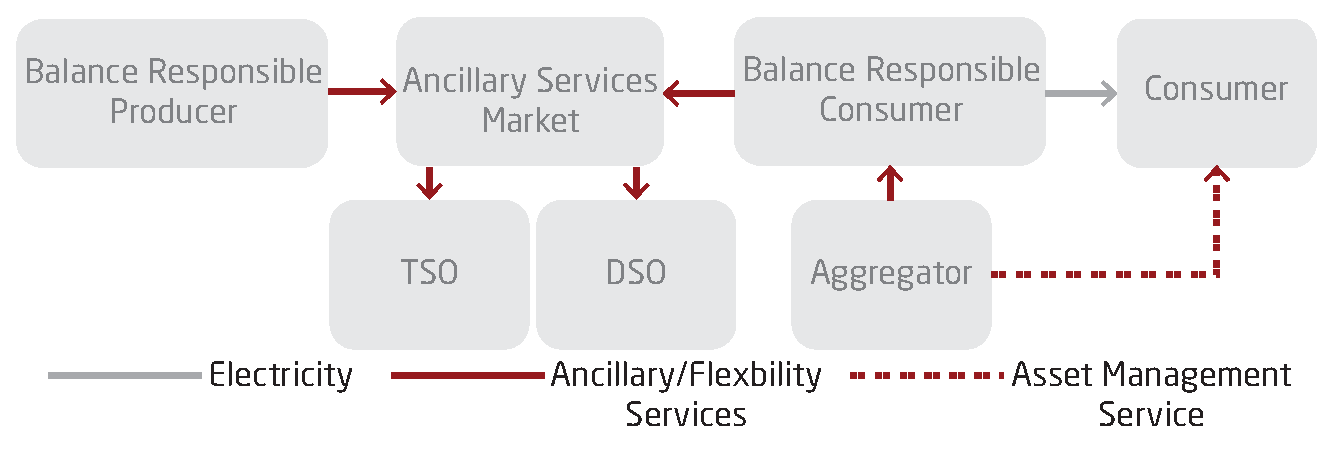
\includegraphics[width=\columnwidth]{graphics/tsg/market_future4}
  \caption{The new player in the market for ancillary services is the aggregator, which sells consumption flexibility on the ancillary service markets through the Balance Responsible Consumer. Some markets allow the aggregators to participate directly in the ancillary service markets with the condition that they coordinate with their Balance Responsible Consumer. It also provides flexibility services to BRPs and DSOs.}
  \label{fig:TSGmarket}
\end{figure}
%The aggregator will sign contracts with the DER owners and be the responsible party for delivery of service to the TSO, DSO or BRP. Further, the aggregator will have to ensure that certain performance parameters are respected towards the DER owner \cite{ding2013development}.
%Introduction of FLECH. \newline

\subsection{Service verification today}
When contracted for service, units are subject to a set of requirements. First, units must pass a prequalification test.% In PJM, when contracted for regulation, this consists of passing three consecutive tests.
Second, certified metering instrumentation must be installed on the unit, and telemetry equipment must be installed and connected to the system operator's Supervisory and Control Data Acquisition (SCADA) system.

For verifying reserve services, the system operator does random checks to see if the reserve is available at the unit \cite{EnerginetAncillary}. %\bondy{I'm not sure who to cite here... in ENDK AS document it is written that ENDK has the right to do random function checks, and that at any moment ENDK can ask for documentation of delivered service... but I've only had it from word of mouth that they actually sometimes do those random tests}\kh{but that's perfect - it's written that they can do it.}
With respect to regulation services, these are expected to be delivered within the required time requirements, and must be measured with acceptable accuracy. For example, for consumption units smaller than 1.5 MW acceptable accuracy is 2\% of the load \cite{Energinettek}.

%``service level agreements´´ etc.
%\kh{here should be a short outline of the actual service verification process; and how it's done today: pre-qualification, certified metering equipment on each generator , , then occasional (?) checks on the response; penalties for non-delivery, etc-}

\subsection{The need for service requirements modeling}\label{subsec:needforreq}
The concept of verification of ancillary services is moving towards a more flexible definition. Furthermore, new types of flexibility services are appearing, e.g. \cite{tougaard2015flech,heussen2013clearinghouse}. Part of the lessons learned from a demonstration of one of these new DSO services \cite{ipowerdemo,bondy2014powermax} is that the services, along with their requirements, need to be clearly defined if aggregators are to deliver them. The main problem being that the verification of services delivered by aggregators is complex.
%\hl{This is because it cannot be assumed that the services will be delivered by traditional (well understood) units, making verification more complex.} 
Also, research points at the need for change of the traditional service requirements if aggregators are to be enabled \cite{macdonald2012demand,koliou2014demand}. Thus, models that translate service contract requirements into benchmarks for performance assessment are needed.

From the market setup described in the previous section, parallels can be drawn to the concept of \emph{Service-Oriented Architectures} (SOAs) from the field of computer science. Under that paradigm, service is defined as: a logical representation of a repeatable business activity that has a specified outcome, is self-contained, may be composed of other services and is a \emph{black box} to consumers of the service \cite{opengroupsoa}. An element in SOAs are \emph{Standardized service contracts}, which contain service level agreements (SLAs). The SLAs can be interpreted as the requirements defined in an ancillary service contract. SLAs must define service performance metrics with corresponding service level objectives (SLOs), which are the agreed means for measuring performance.
%\kh{here motivate the need for formalized and generic requirements; good to use the iPower experience here as motivation}

PJM has established precedence in using performance metrics for verification of services. Their \emph{performance score} consists of a weighted average of three measures: delay, accuracy and precision. These measure the delay and correlation between the regulation signal and the reaction of the unit, and the difference in energy requested vs. energy supplied \cite{pjmperf}. These measures are tailored to the way frequency regulation is done at PJM (tracking of the regulation signal). Therefore, more general (and simple) models and performance metrics are needed to cover other frequency regulation services and the new flexibility services.


\section{Method for service modeling}\label{sec:methodology}
Currently, services requirements are defined in a contract, but there is no standardized method for transforming contractual requirements into a mathematical model (requirements model) that a computer can use for verification of service delivery. This requirements model forms the base-line against which the delivered service is benchmarked. The model incorporates both the ideal and acceptable service provision. By analysis of the TSO services defined in \cite{EnerginetAncillary}, the potential DSO services defined in \cite{ding2013development} and asset management services, we have developed a method for modeling the service delivery over time. 
%The method presented in this section outlines the steps to transforming contractual requirements into a requirements model.
The method consists of the following six steps:
%form have been identified as a generic method for modeling ancillary services. The steps are exemplified by DSO services defined in  and TSO services defined in :
\begin{enumerate}
  \item Identify physical parameters defining the service.
%  \begin{itemize}
%    \item For example: Power production or consumption, measured grid frequency, time measurements. Including maximum measuring sensitivities.
%  \end{itemize}
  \item Identify the dynamic behaviors of the service related to system parameters (if any).
%  \begin{itemize}
%    \item Example: Primary frequency regulation comes with a linear behavior between grid frequency and generator set-point. Power-cap has a dynamic relationship between feeder load and the controllable load power in order to keep the total feeder load at a $P_{DSO,Ref}$ value.
%    \item PowerMax is not dynamic. The aggregator must control $\Delta P_{Agg}$ to ensure that he does not violate $P_{max,Agg}$. But the service does not require a dynamic behavior related to a system parameter like primary frequency regulation and PowerCap.
%  \end{itemize}
  \item Identify the physical size of the service and the tolerated error. % Both ideal service and minimum required service.
%  \begin{itemize}
%    \item Physical size is for example $P_{max,Agg}$ for PowerMax service or regulation bid for primary frequency regulation.
%    \item Tolerance is for example $P_{max,Agg}+P_{tolerance}$ for the PowerMax service and allowed dead-band for DK1 primary reserve.
%  \end{itemize}
  \item Identify the ideal response time of the service and acceptable response.
%  \begin{itemize}
%    \item Most contracts comes with some timing specifying how fast the service provider must act.
%    \item E.g. DK1 primary reserve must provide 50 \% of service within 15 s and 100 \% within 30 s.
%    \item The ideal service is for example an instantaneous step in power to 100 \% of set-point for DK1 primary reserve.
%  \end{itemize}
  \item Based on the dynamics, size and timing of the service, as well as the tolerated errors from points 1--4, develop a time series for ideal and acceptable service provision. The model will be a set of time series: $\mathbf{x}_{ideal}(t)$ for ideal response and $\mathbf{x}_{acc}(t)$ for acceptable response. Both time series can be a scalar or a vector, e.g. $\mathbf{x}_{acc}(t)$ can be formed by a set of upper and lower tolerance bounds or simply by an upper bound.
  %§$\mathbf{x}_{ideal}(t)$ and $\mathbf{x}_{acc}(t)$ can be a pair of values, e.g. minimum and maximum tolerance limits, for some services and may be only a single value, e.g. minimum or maximum tolerance, for others. 
  \item Identify how the service error is to be measured.
\end{enumerate}

We identify three different types of service: reference tracking, band service or a maximum/minimum cap. The error measure, $e(t) \in \mathbb{R}$, for each of the service types is defined in the following subsections. This approach was initially introduced in \cite{bondy2014performance}, and is further refined in this work. 

%The error, $e(t) \in \mathbb{R}$, in the delivery of a service can be calculated using a reference tracking, band service or a maximum/minimum cap approach. The proposed approach depends on the specific service and contract.\bondynote{These last two paragraphs can probably be merged}


\subsection*{Reference tracking}
Reference tracking error can be calculated as:
\begin{equation}\label{eq:ref_error}
e(t) = x_{meas}(t) - x_{ideal}(t).
\end{equation}
This definition will lead $e<0$ for measured values below the ideal and $e>0$ for values above the ideal. In this case $\mathbf{x}_{acc}(t)$ will be a band around $x_{ideal}(t)$, and the values of $\mathbf{x}_{acc}(t)$ do not need to be symmetric.

\subsection*{Band service}
The ideal response in a band service is defined as $ \mathbf{x}_{ideal}(t)= [x_{min}(t),x_{max}(t)]$. The error in the band service can therefore be estimated by:
\begin{equation}\label{eq:band_error}
e(t)=
\begin{cases}
x_{meas}(t) - x_{min}(t) , & x_{meas}(t) < x_{min}(t)  \\
0, & x_{min}(t) \leq x_{meas}(t) \leq x_{max}(t) \\
x_{meas}(t) - x_{max}(t), & x_{meas}(t)  > x_{max}(t).  
\end{cases}
\end{equation}
In this case, the $\mathbf{x}_{acc}(t)$ is a set of values that surrounds the band defined by $ \mathbf{x}_{ideal}(t)$, as seen in Fig.~\ref{fig:RefErr}. The values of $\mathbf{x}_{acc}(t)$ do not need to be symmetric around the band.

\subsection*{Cap service}
%Maximum/minimum cap error only counts the error when performance is above/below some ideal value. 
In cap services, error is only tracked when $x_{meas}(t)$ is either above or below a given a limit value.
Maximum cap error is calculated as shown in \eqref{eq:maxmin_cap} and minimum cap can be similarly calculated. In \eqref{eq:maxmin_cap}, $x_{max}(t)$ is the ideal maximum limit according to the service contract:

\begin{equation}\label{eq:maxmin_cap}
e(t)=
\begin{cases}
x_{meas}(t)-x_{max}(t), & x_{meas}(t) > x_{max}(t) \\
0, & x_{meas}(t) \leq x_{max}(t).
\end{cases}
\end{equation}
In the cap service, $x_{acc}(t)$ is a limit that either lies below $x_{min}(t)$ or above $x_{max}(t)$.

Having defined the method for formulating the service models, we will show how these can be used for performance assessment of services.


\section{Performance Assessment of Service Delivery}\label{sec:performance}
%\kh{this paragrpah has an apologetic tone ... }
In Sec.~\ref{subsec:needforreq} three requirements for performance metrics are presented. These can be expressed formally as:
\begin{align}
    \text{[P-R1]:} \quad & \eta = f_P(x_{meas},\mathbf{x}_{acc},t), \quad \eta \in [0,1],\\
    \text{[P-R2]:} \quad & \epsilon = f_R(x_{meas},\mathbf{x}_{acc},t),\\
    \text{[P-R3a]:} \quad & \eta_K = \sum_{i \in M} f_M(\eta_i), \quad \eta_i \in [0,1],\\
    \text{[P-R3b]:} \quad & \epsilon_M = \sum_{i \in M} f_M(\epsilon_i),\\
\end{align}
where $\eta$ is a quality performance measure, $\epsilon$ is a reliability measure, $\eta_M$ and $\epsilon_M$ are the same measures applied to multiple services \emph{M}. The measured output (or sum of outputs in the case of aggregation) is defined by $x_{meas}$, and the service bounds are defined by $\mathbf{x}_{acc}$, as defined in Sec.~\ref{susec:reqmodform}. $f_P(\cdot)$ is a function that evaluates service performance normalized to $\mathbf{x}_{acc}$ and time \emph{t}. Similarly, $f_R(\cdot)$ is a function that evaluates service reliability based upon $\mathbf{x}_{acc}$ and normalized to time and $f_M(\cdot)$ is a function that gives an overall measure for multiple services.

These concepts were originally presented in \cite{bondy2014performance}, but are revised and expanded upon following concepts from \cite{thavlov2015thesis}. In order to asses service performance three concepts are introduced in this section:
\begin{itemize}
\item Quality of Service, which is an instantaneous measure of how well the aggregator is delivering one service within the contract constraints;
\item service performance assessment index, which describes the overall performance of the aggregator over the delivery period for the services, or subset of services, it is providing; and a
\item service verification index, which describes how much an aggregator is breaking the contractual agreements (non-delivering) of the services, or a subset of services, it provides.
\end{itemize}

Differently from the previous work, the service delivery index is split into measures of the ancillary services (AS) delivered to system operators and the AMS delivered to unit owners (see Sec.~\ref{subsec:ASDER}). In this way, a system operator (or a third party certification company) can use the index for certification of aggregators, for which the AMS evaluation is irrelevant. Furthermore, the service verification index is introduced, and a new way of defining the quality of service is presented.
%\athanote{We should be a bit more explicit about services delivered upwards in the system (AS) and down-wards (AMS) to the asset owner}

\subsection{Quality of Service}
Quality of service (QoS) is a measure defined in \cite{bondy2014performance}, where it is used to assess the quality of a power system service at any given time. QoS at any given time is given by:
\begin{equation}\label{eq:QoS}
QoS(t)=e(t)C_{n}(t)
\end{equation}
where \emph{e(t)} is the error in service delivery introduced in Sec.~\ref{sec:TSGmethodology}, and $C_n(t)$ is a normalization factor that can be time varying. Following [P-R1], we define:
\begin{itemize}
\item $QoS \geq 0$;
\item for $QoS \leq 1$ the service is considered delivered within the contractual constraints;
\item and $QoS = 0$ is a perfect service delivery.
\end{itemize}
In order to achieve these definitions, the normalization factor $C_{n}(t)$ must be calculated from $\mathbf{x}_{acc}(t)$ thus:
\begin{equation}
C_{n}(t) = 
\begin{cases}
\frac{1}{x_{acc,max}(t) - x_{max}(t)}, & e(t) \geq 0 \\
\frac{1}{x_{acc,min}(t) - x_{min}(t)}, & e(t) < 0.
\end{cases}\label{eq:cst}
\end{equation}
where $x_{acc,max/min}$ and $x_{max/min}$ are part of the service model defined in Sec.~\ref{sec:TSGmethodology}. By defining $C_{n}(t)$ in this way, we take into account the possibility of asymmetry in the values of $x_{acc}$, and ensure that QoS is a positive value. A visual representation of this scaling can be seen in Fig.~\ref{fig:TSGtracking_error}--Fig.~\ref{fig:TSGcap_error}, where the QoS for the three kinds of services are presented.
In general, the rate with which $QoS(t)$ increases depends on the difference between $x_{acc}(t)$ and $x_{ideal}(t)$.
\begin{figure}
\centering
\subfloat[Error]{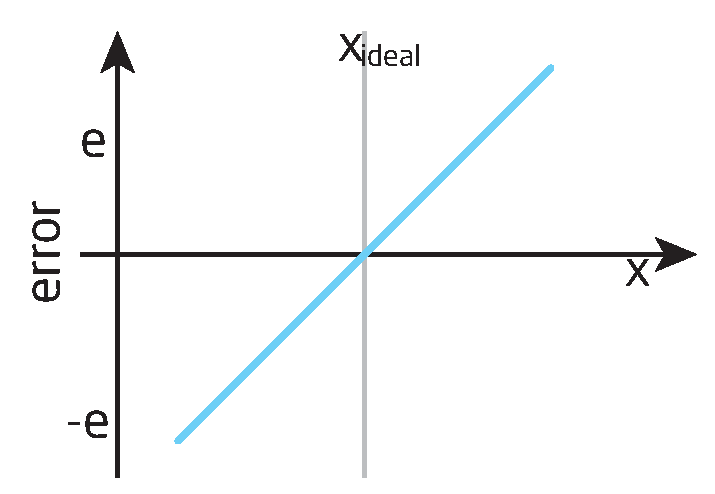
\includegraphics[width=0.5\columnwidth]{graphics/tsg/tracking_error2.eps}%
\label{fig:errortracking}} \subfloat[Quality of Service]{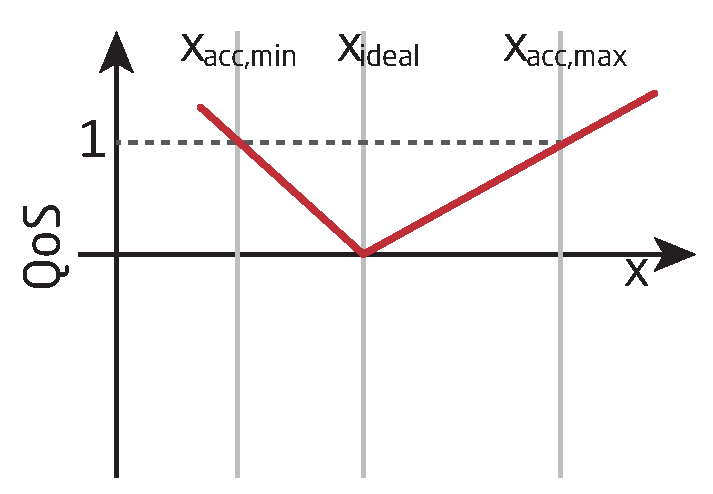
\includegraphics[width=0.5\columnwidth]{graphics/tsg/tracking_error3.eps}%
\label{fig:qostracking}}
\caption{Error and QoS for tracking services, note that the acceptable band do not need to be symmetric.}
\label{fig:TSGtracking_error}
\end{figure}
\begin{figure}
\centering
\subfloat[Error]{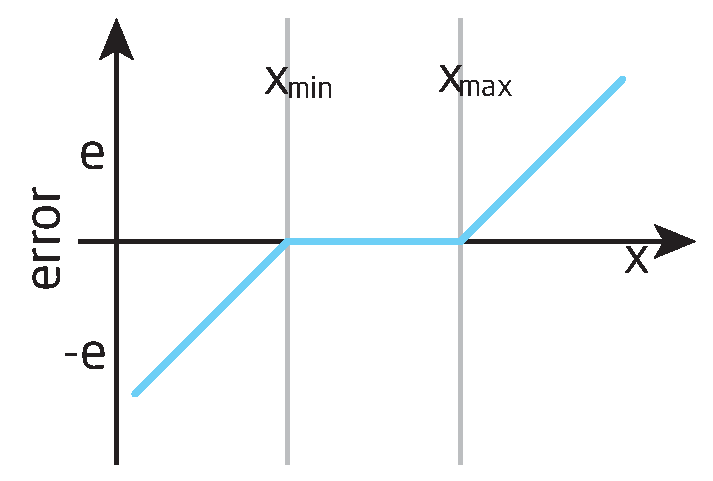
\includegraphics[width=0.5\columnwidth]{graphics/tsg/band_error2.eps}%
\label{fig:errorband}}\subfloat[Quality of Service]{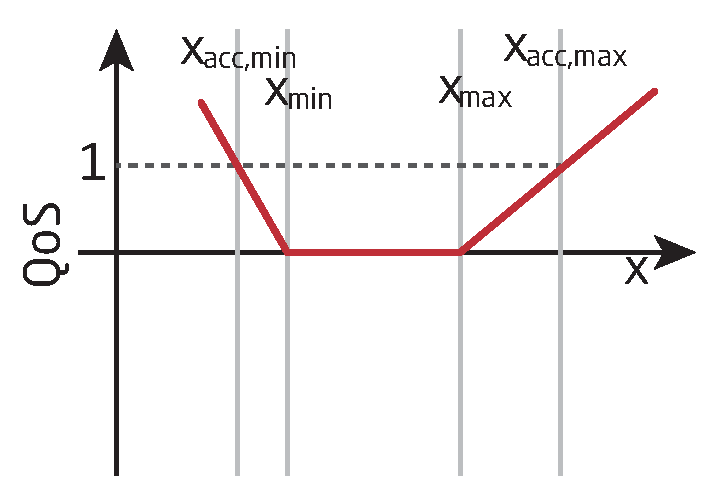
\includegraphics[width=0.5\columnwidth]{graphics/tsg/band_error3.eps}%
\label{fig:qosband}}
\caption{Error and QoS for band services.}
\label{fig:TSGband_error}
\end{figure}
\begin{figure}
\centering
\subfloat[Error]{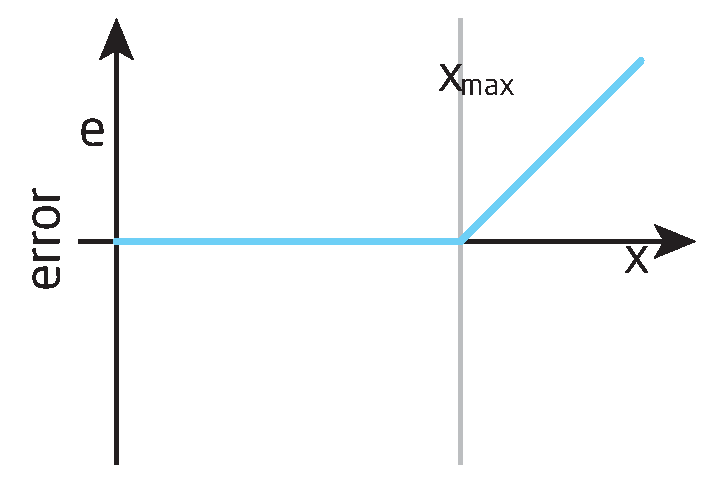
\includegraphics[width=0.5\columnwidth]{graphics/tsg/cap_error2.eps}%
\label{fig:errorcap}}
\subfloat[Quality of Service]{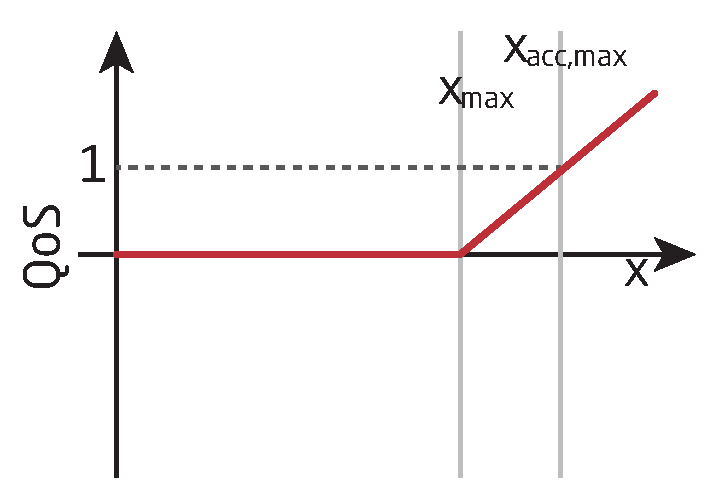
\includegraphics[width=0.5\columnwidth]{graphics/tsg/cap_error3.eps}%
\label{fig:qoscap}}
\caption{QoS for a maximum cap service, a minimum cap service is defined similarly but with $x_{min}$ and $x_{acc,min}$ values.}
\label{fig:TSGcap_error}
\end{figure}
%\begin{figure*}[!t]
%\centerline{\subfloat[Case I]\includegraphics[width=2.5in]{subfigcase1}%
%\label{fig_first_case}}
%\hfil
%\subfloat[Case II]{\includegraphics[width=2.5in]{subfigcase2}%
%\label{fig_second_case}}}
%\caption{Simulation results}
%\label{fig_sim}
%\end{figure*}

Note that in \eqref{eq:cst}, $C_{n}(t)$ is not defined for $x_{acc}(t) = x_{ideal}(t)$. This is a corner case, in which:
%\bondynote{This QoS is only used then to calculate the Non-Delivery K, so, since we subtract 1 later on anyway, we might as well say the cornercase automatically starts counting on the Non-Delivery, and QoS = 1 for $e \neq 0$}
\begin{equation}
QoS(t) = e(t), \quad x_{acc}(t) = x_{ideal}(t)
\end{equation}


\subsection{Assessing service delivery}
Based on the above instantaneous measure for the quality of individual services, we can evaluate the aggregator as a whole based upon the quality of all the services it delivers. 

%\khnote{formalized requirements here}

The overall service delivery index of AS is defined by $\eta^{AS}$ in Eq.~\eqref{eq:TSGetaAS}, but before calculating the index, the non-delivery incidents (which are measured apart) must be sorted out. This is done by restricting $QoS_{K,meas}^{AS}(t)$ (the measured quality of service for the \emph{K} ancillary services the aggregator is providing) such that it does not account for $QoS > 1$: 
%\begin{algorithmic}[H]
%\FOR{ t = 0:$t_N$ }
%\FOR{ i = 1:K}
%    \IF{$QoS_{i,meas}^{AS}(t)>1$} 
%        \STATE $QoS_{i}^{AS}(t) = 1$ 
%    \ELSE 
%        \STATE $QoS_{i}^{AS}(t) = QoS_{i,meas}^{AS}(t)$
%    \ENDIF
%\ENDFOR
%\ENDFOR
%\end{algorithmic}
\begin{align}
	QoS^{AS}(t) = \begin{cases} QoS^{AS}_{meas}(t) ,\quad &\forall QoS^{AS}_{meas}(t) \leq 1, \forall t\\
	1, \quad &\forall QoS^{AS}_{meas}(t) > 1, \forall t.
	\end{cases}
\end{align}

where \emph{K} is the total number of AS the aggregator provide.
This restriction is not done in \cite{bondy2014performance} since that work did not use a separate reliability index. This means that $\eta_{AS}$ is only a measure of the service provision performance within the contractual limits.

While the previous definitions have been established in continuous time, the actual measurement and calculations are done in discrete time. This leads to $\eta_{AS}$ being estimated for \emph{K} amount of AS over each corresponding discrete time horizon $N_K$:
\begin{align}\label{eq:TSGetaAS}
\eta^{AS} &= \sum^{K}_{i=1} W_i \sqrt{\frac{\sum^{N_i}_{t=0} \left( {QoS^{AS}_{i,t}}^{2} \right)}{N_i}}\\
\sum_{i=1}^K W^{AS}_i &= 1
\end{align}
where $W^{AS}_K$ is the assigned weight to each AS, leading to $\eta^{AS} \in [0,1]$, and $\eta$ close to zero representing good performance while $\eta$ close to 1 representing a barely acceptable performance. This means that the service performance assessment index for all the AS the aggregator provides is a weighted average of the root mean square (RMS) of the error in all service deliveries, thus satisfying [P-R3a]. With this index it is possible to evaluate aggregators that deliver more than one AS at a time, e.g. a frequency containment reserve and a replacement reserve, and assign a hierarchy of importance with respect to the services. However, how to do distinguish measurements to verify the services, and how to evaluate which service is more important, is out of scope of this work, but the definition of Eq.~\eqref{eq:TSGetaAS} takes the possibilities into account. In the case where only a single service delivery is considered, Eq.~\eqref{eq:TSGetaAS} is simply the RMS of the error in service delivery:
\begin{equation}\label{eq:etaASsimp}
\eta^{AS} = \sqrt{\frac{\sum^{N}_{t=0} \left( {QoS^{AS}_{t}}^{2} \right)}{N}},
\end{equation}
which satisfies [P-R1]. 

Eq.~\eqref{eq:TSGetaAS} gives an idea of the performance of the aggregator where the duration of time delivery is taken into account. This means that two service provisions are evaluated equally when their error in service delivery compared to the duration of the service delivery are the same. %With these definitions, requirements \emph{R1}, \emph{R2} and \emph{R4} are fulfilled.

%Similarly, the ability of the aggregator to deliver AMS as a whole can be measured with an index $\eta^{AMS}$ (Eq.~\eqref{eq:etaAMS}). In this instance, QoS is also clamped to $QoS^{AMS}_{M}(t) \in [0,1]$, and the amount of \emph{M} services are evaluated for their corresponding time horizon $N_M$:
%\begin{equation}\label{eq:etaAMS}
%\eta^{AMS} = \sum^{M}_{i=1} W^{AMS}_i \sqrt{\frac{\sum^{N_i}_{t=0} \left( {QoS^{AMS}_{i,t}}^{2} \right)}{N_i}}
%\end{equation}
%with $\eta^{AMS} \in [0,1]$ and $\sum_{i=1}^M W^{AMS}_i = 1$. Each of 

%Finally, if the aggregator desires to have an internal overall evaluation of all the services it is providing, it can do so through a weighted mean of the service performance indices:
%\begin{equation}
%\eta_{tot} = \alpha \eta^{AS} + (1-\alpha) \eta^{AMS}, \quad \alpha \in [0,1]
%\end{equation}
%where $\alpha$ is the weight ratio the aggregator assigns to the performance of the services.

\subsection{Verifying service delivery}
Requirement \emph{P-R2} defines a reliability measure. To address this requirement, an index $\epsilon^{AS}$, similar to the service performance assessment index, is defined for verifying the delivery of AS\footnote{This can also be interpreted as evaluating non-delivery of service.}. Also, a non-delivery measure for the AS provision, $ND^{AS}$, is defined according to the expression:
\begin{align}
	ND^{AS}(t) = \begin{cases} QoS^{AS}_{meas}(t) - 1,\quad &\forall QoS^{AS}_{meas}(t) > 1, \forall t\\
	0, \quad &\forall QoS^{AS}(t) \leq 1, \forall t.
	\end{cases}\label{eq:ndasclamp}
\end{align}
%\begin{algorithmic}[H]
%\FOR{ t = 0:$t_N $}
%\FOR{ i = 0:K}
%    \IF{$QoS^{AS}_{i,meas}(t)<1$} 
%        \STATE $ND^{AS}(t) = 0$ 
%    \ELSE 
%        \STATE $ND^{AS}(t) = QoS^{AS}_{i,meas}(t)-1$
%    \ENDIF
%\ENDFOR
%\ENDFOR
%\end{algorithmic}
Eq.~\eqref{eq:ndasclamp} shows that whenever the QoS of a service exceeds 1, i.e. the limit of what is an acceptable service provision, the amount with which it breaks the acceptable constraint is measured by \emph{ND}.
$\epsilon^{AS}$ is calculated in the same way as $\eta^{AS}$ using $ND^{AS}_K(t)$ instead of $QoS^{AS}_{K}(t)$:

\begin{equation}\label{eq:TSGepsilonAS}
\epsilon^{AS} = \sum^{K}_{i=1} W_i \sqrt{\frac{\sum^{N_i}_{t=0} \left( {ND^{AS}_{i,t}}^{2} \right)}{N_i}}
\end{equation}
where $\epsilon^{AS} \in [0,\infty]$. This expression satisfies [P-R3b], and in the case where \emph{K=1} it also satisfies [P-R2].

%Similarly, the non-delivery measure of the AMS $\epsilon^{AMS}$ is defined as:
%\begin{equation}\label{eq:epsilonAMS}
%\epsilon^{AMS} = \sum^{M}_{i=1} W_i \sqrt{\frac{\sum^{N_i}_{t=0} \left( {ND^{AMS}_{i,t}}^{2} \right)}{N_i}}.
%\end{equation}

Thus, $\epsilon$ is used to asses the severity of non-delivery events. For some systems it is critically important that $QoS(t)\leq1$ at any time, in which case $\epsilon$ should be close to zero for the contract to be considered respected. Other systems can tolerate $QoS(t)>1$ for some period, which leads to a higher acceptable $\epsilon$. A service delivery is verified if $\epsilon \leq \epsilon_{max}$, and this contractual limit, i.e. the value of $\epsilon_{max}$, must be assessed individually depending on the nature of the system. %It is likely that in most cases $\epsilon^{AS}_{max}<\epsilon^{AMS}_{max}$, since the security of the power system is more important than, e.g., the temperature comfort of a home owner.

In \cite{bondy2014performance}, non-delivery is assesed using a non-delivery counter (NDC). $\epsilon$ differs from the NDC in that it both captures the time span of non-delivery and the magnitude of the violation, whereas NDC only captures the amount of time samples where non-delivery is detected. $\epsilon$ might prove advantageous over the NDC as a service verification index for some systems. A disadvantage of $\epsilon$ is that it might be a less intuitive measure to communicate to the service providers compared to the NDC.

Fig. \ref{fig:RefErr} shows an example of reference tracking error service performance assessment. Deviations between $x_{meas}$ and $x_{ideal}$ inside the band defined by $x_{acc}$ will lead to $QoS<1$, while deviations outside the $x_{acc}$ band will lead to $QoS>1$. For this particular example $\eta^{AS}=0.7501$ and the service verification index is $\epsilon^{AS}=0.2324$, which indicates that generally the service provision is bad at following the reference, and also has a moderate amount of non-delivery. The service acquirer will have to decide whether this verification index value is acceptable or if it should lead to economical penalization or contract termination.

\begin{figure}
\centering
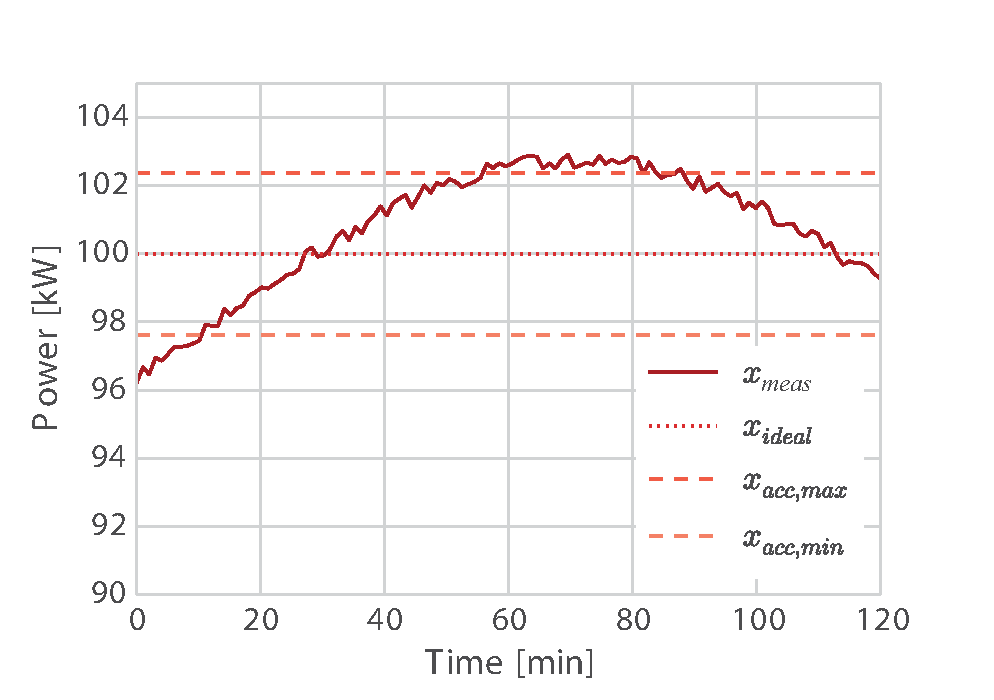
\includegraphics[width=\columnwidth]{graphics/tsg/reftrack2.eps}
\caption{Example of reference tracking error with performance $x_{meas}$, ideal performance $x_{ideal}$ and tolerance limits $x_{acc}$.}
\label{fig:RefErr}
\end{figure}


\section{Case Studies}\label{sec:casestudies}
Using two different ancillary services and an asset management service as cases, we will illustrate the utility of the generic service modeling method, the service performance index and the service verification index. The first case study focuses on frequency containment reserve in western Denmark, the second focuses on the theoretical PowerMax DSO service, and the third focuses on the temperature management of a residential house. 

\subsection{Frequency Containment Reserve in Western Denmark}
Frequency Containment Reserve (FCR) is utilized to contain frequency excursions deviating from the nominal 50 Hz in \emph{ENTSO-E RG Continental Europe’s synchronous area} of which western Denmark (DK1) is part of. The Danish TSO, Energinet.dk, is obliged to provide a proportional share of $\pm$ 23 MW \cite{EnerginetAncillary} out of the total synchronous area need of $\pm$ 3000 MW. Energinet.dk buys these reserves at daily auctions. The service specifications are defined in \cite{EnerginetAncillary}.

The six steps outlined in Sec.~\ref{sec:SEGANmethodology} are used to model the ideal and tolerated service response. 1) The physical parameters are grid frequency (accuracy of $\pm$ 10 mHz or better), generator reserve power output, and timing of service delivery (accuracy of 1 s or better). 2) The reserve must be supplied linearly at deviations of $\pm$ 200 mHz relative to 50 Hz, with a $\pm$ 20 mHz dead-band around 50 Hz. 3) The physical size of the service depends on the reserve bid size. This work will look at a generic reserve bid. According to the discussion from Eq.~\eqref{eq:QoS}, $x_{ideal}$ cannot be equal to $\mathbf{x}_{acc}$. Therefore, a $\pm$ 1\% tolerance band of $x_{ideal}$ is assumed. 4) The first 50\% of the service must be supplied within 15 s and 100\% must be supplied within 30 s. The ideal response can be defined as a response with an instant 100\% power ramp \cite{makarov2008assessing}. 5) The ideal and tolerated response of this service provision is plotted as $x_{ideal}$, $x_{acc,min}$ and $x_{acc,max}$ in Fig.~\ref{fig:DK1PrimResSim}, which assumes that a reserve power set-point has already been established based on the values from step 2.%Fig.~\ref{fig:DK1PrimResDyn}

%\begin{figure}
%\centering
%\includegraphics[width=\columnwidth]{figures/dynresp.eps}
%\caption{DK1 Primary Reserve service provision curve. The curve shows the relationship between the activated fraction of the primary reserve bid, and the grid frequency, including the +/- 20 mHz dead-band. This should not be confused with the droop curve.}
%\label{fig:DK1PrimResDyn}
%\end{figure}

Fig. \ref{fig:DK1PrimResSim} shows a simulation of primary regulation active power ramp $x_{act}$ for the time interval $[-5,35]$ s. The service delivery performance index and non-delivery verification index are $\eta^{AS}=0.4257$ and $\epsilon^{AS}=0.1392$, calculated using Eq. \eqref{eq:etaAS} and Eq.~\eqref{eq:epsilonAS}. The TSO must determine a threshold $\epsilon_{max}$, such that the service provider is penalized or the contract is terminated if $\epsilon^{AS}>\epsilon^{AS}_{max}$. It is not the scope of this work to asses a suitable value of $\epsilon^{AS}_{max}$.%\bondynote{We are repeating ourselves a bit here}

\begin{figure}
\centering
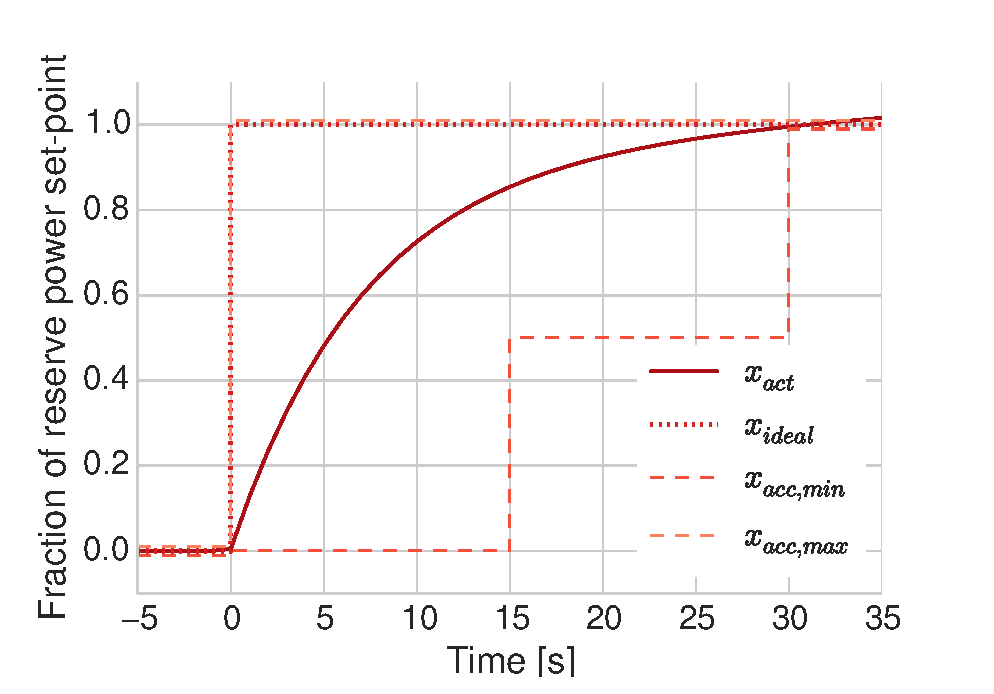
\includegraphics[width = \columnwidth]{SEGAN/primfreqresp.eps}
\caption{Simulation of a DK1 primary reserve power ramp response together with $x_{ideal}$ and $x_{acc}$ values.}
\label{fig:DK1PrimResSim}
\end{figure}

\subsection{PowerMax in a distribution system}
The \textit{PowerMax} service was first described in \cite{ding2013development} and further specified in \cite{bondy2014flech}. It is a DSO service, where the DSO can make a tender for a load reduction $\Delta P^{DSO}$ to a max level $P_{max}^{DSO}$ in parts of the distribution system that are forecasted to experience congestions during some periods (e.g. hours 17-20 during winter months). The motivation for \textit{PowerMax} is that the service could be an economically beneficial alternative to grid reinforcements in some situations. This is both due to saved interest and depreciation on investments plus the avoided risk of over-sizing equipment in case of future energy savings or if the disappearance of a large consumer makes the reinforcement unnecessary.% The tender is announced and cleared through Flexibility Clearing House (FLECH), where flexibility aggregators can bid on the tender.%where the service is delivered by aggregator companies, which bid in flexibility from a group of units which they control. 

%Following is a mathematical definition of the \textit{PowerMax} service, as previously developed in \cite{bondy2014powermax}. 
In order to identify its service needs, it is assumed that the DSO is able to separate the total consumption forecast $\hat{P}_{tot}$ in the congested part of the distribution grid into a controllable load forecast $\hat{P}_{CL}$ and a base load forecast $\hat{P}_{BL}$:
\begin{align}
\hat{P}_{tot} &= \hat{P}_{CL} + \hat{P}_{BL} \\
\hat{P}_{CL} &= \sum_{Agg} \hat{P}_{CL,Agg}, \quad Agg \in \mathbf{A} \label{eq:CLDef}
\end{align}
where $\mathbf{A}$ is the set of all aggregators in the considered part of the grid. Only the aggregators \emph{Agg} that bid for the service tender make up $\hat{P}_{CL}$, while the rest of $\mathbf{A}$ is part of $\hat{P}_{BL}$. The aggregators must be contracted to deliver a total power reduction $\Delta P$, such that the system operational limit $\bar{P}_{sys}$ is not violated by the peak base load forecast and the peak controllable load forecast:

\begin{equation}
\hat{\bar{P}}_{BL}+\hat{\bar{P}}_{CL}-\Delta P \leq \bar{P}_{sys}. \label{eq:PSysDef}
\end{equation}

This inequality can be fulfilled by setting a peak limit $\bar{P}_{CL}$:
\begin{equation}
\bar{P}_{CL} = \hat{\bar{P}}_{CL} - \Delta P \label{eq:PBarCLDef}
\end{equation}
where $\Delta P$ and $\bar{P}_{CL}$ are the variables for the DSO service tender. In order to formulate a service tender, the magnitude of these variables must be estimated taking into account the uncertainty of the forecasts, giving the following expressions:
\begin{align}
\Delta P^{DSO} &= \sum_{Agg} \Delta \hat{P}_{CL,Agg} + \text{Risk\{}\hat{P}_{CL} + \hat{P}_{BL}\text{\}}\\
P_{max}^{DSO} &= \hat{\bar{P}}_{CL} - \Delta P_{DSO}
\end{align}
where $\Delta \hat{P}_{CL,Agg}$ is the estimated power reduction for the individual aggregator bid, $\text{Risk\{}\hat{P}_{CL} + \hat{P}_{BL}\text{\}}$ is the risk associated to the load forecast uncertainty. $Agg \in \mathbf{A_{C}}$ and $\mathbf{A_{C}} \subseteq \mathbf{A}$, i.e. $\mathbf{A_{C}}$ is the subset of aggregators that bid on the tender. After the DSO has identified a suitable $P_{max}^{DSO}$ and $\Delta P^{DSO}$ to solve the congestion issue, the DSO formulates a service tender for which aggregators can bid their corresponding $\Delta P^{Agg}$ and $P^{Agg}_{max}$. %The DSO sets a maximum price it is willing to pay for the load reduction, which is related to the alternative cost of grid reinforcements. In case the market is not cleared at or below the maximum price, the DSO can formulate a new tender, adjusting the risk value, POD (point of delivery) list or amount of power reduction. The timing of the tender process should be such that the DSO has time to conduct grid reinforcements as an alternative.

The method from Sec.~\ref{sec:SEGANmethodology} is used to model \textit{PowerMax} ideal and acceptable response. 1) The physical parameters are $P_{max}^{Agg}$, $\Delta P^{Agg}$ and months/days/hours the service shall be delivered. 2) The system does not posses a dynamic behaviour related to system parameters. 3) As an example, the service tender defines $P_{max}^{Agg} = 200$ kW and $+1\%$ allowed deviation $P_{max,acc}^{Agg}$. 4) In this example we use 120 min service provision time with allowed non-delivery in the first 15 min, and the last 5 min, of the service delivery (following the service definition in \cite{ding2013development}) and the ideal service delivery is the one that respects $P_{max}^{DSO}$. 5) Figure \ref{fig:PowerMaxSim} plots $x_{ideal}$ and $x_{acc}$. The \textit{Activation Dead-band} indicates the regions where the aggregator is not obliged to deliver the service because of the tolerances defined under step 4. 6) The service is a maximum cap service and the error is measured as in Eq.~\eqref{eq:maxmin_cap}.

An example of a load curve $P_{Agg}=x_{act}$ is presented in Fig.~\ref{fig:PowerMaxSim}. The service delivery and verification are evaluated using Eq.~\eqref{eq:etaAS} and Eq.~\eqref{eq:epsilonAS}, yielding $\eta^{AS} = 0.5074$ and $\epsilon^{AS} = 0.2701$ respectively. As with the performance assessment of the FCR in DK1, it is not within the scope of this paper to asses the value of $\epsilon^{AS}_{max}$, yet a qualified assessment can be made. %, which will lead to either penalization or termination of the contract.
To asses $\epsilon^{AS}_{max}$, the DSO must analyze the dynamics of the problem the service is helping relieve. For \textit{PowerMax}, the dynamics are governed by the heating of the overloaded equipment (e.g. transformer or cable), which deteriorates over time due to overheating. A feeder might be tolerant to short term overloads and therefore the DSO might set $\epsilon^{AS}_{max}$ higher than in the FCR case.

\begin{figure}
\centering
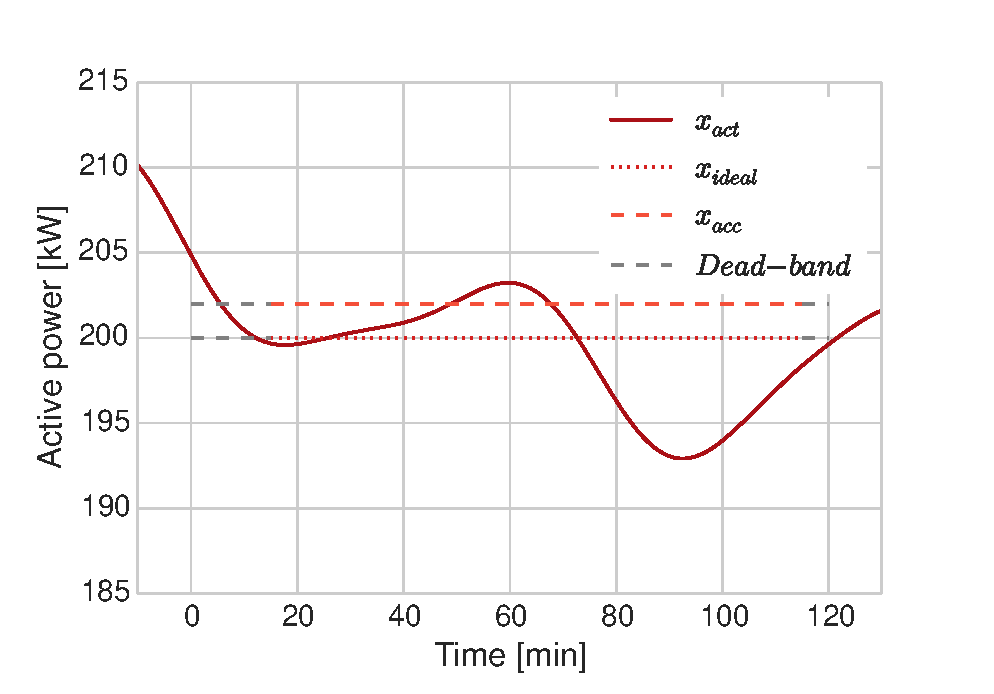
\includegraphics[width = 0.86\columnwidth]{SEGAN/powermaxsample.eps}
\vspace{-4pt}
\caption{$x_{ideal}=P_{max}^{Agg}$, $x_{acc}=P_{max,acc}^{Agg}$ for the considered \textit{PowerMax} example. The activation Dead-band is the time period, where the aggregator is allowed to non-deliver.}\label{fig:PowerMaxSim}
\end{figure}

\subsection{Temperature management of a flexible household}
Household heating is a flexible process where the thermal capacity of the building can be considered a form of energy storage. In Denmark, heat pumps are being installed with the capability of being remotely controlled by an aggregator, see e.g. \cite{insero}. It is assumed that the aggregator will help the heat pump owners to maintain a comfortable indoor temperature and utilize the electric consumption flexibility in exchange of monetary compensation.

Applying the method from Sec.~\ref{sec:SEGANmethodology} to model the service: 1) The physical parameters are the minimum and maximum of the temperature comfort bands of the household. 2) The service does not posses a dynamic behaviour related to system parameters. 3) As an example, the household owner sets a comfort band of $\mathbf{x}_{ideal} = [x_{min},x_{max}] = [20 ^{\circ}\text{C},22^{\circ}\text{C}]$ and allows for a $\pm 1 ^{\circ}\text{C}$ as acceptable error. Furthermore, the owner decides that during the night, the house can be two degrees colder. 4) In this example the ideal response is performance within the temperature bounds. 5) Fig.~\ref{fig:tempband} plots $x_{ideal}$ and $\mathbf{x}_{acc}$. 6) The service is a band service and the error is measured according to Eq.~\eqref{eq:band_error}.

The service model and the actual temperature of a simulation can be seen in Fig.~\ref{fig:tempband}, where it is clear that generally the aggregator is able to provide a reasonable service performance, with no non-delivery ( $\eta^{AMS} = 0.2707$ and $\epsilon^{AMS} = 0.0$). As described in Sec.~\ref{sec:DERs}, the aggregator may be in charge of the overall control of a cluster of units, in which case the performance should be evaluated over the whole cluster. To show this, simulations are done for 20 households and the equally-weighted average of the indices results in $\eta^{AMS} = 0.2411$ and $\epsilon^{AMS} = 0.0211$ (Fig.~\ref{fig:tempbandclustererror}).

\begin{figure}
\centering
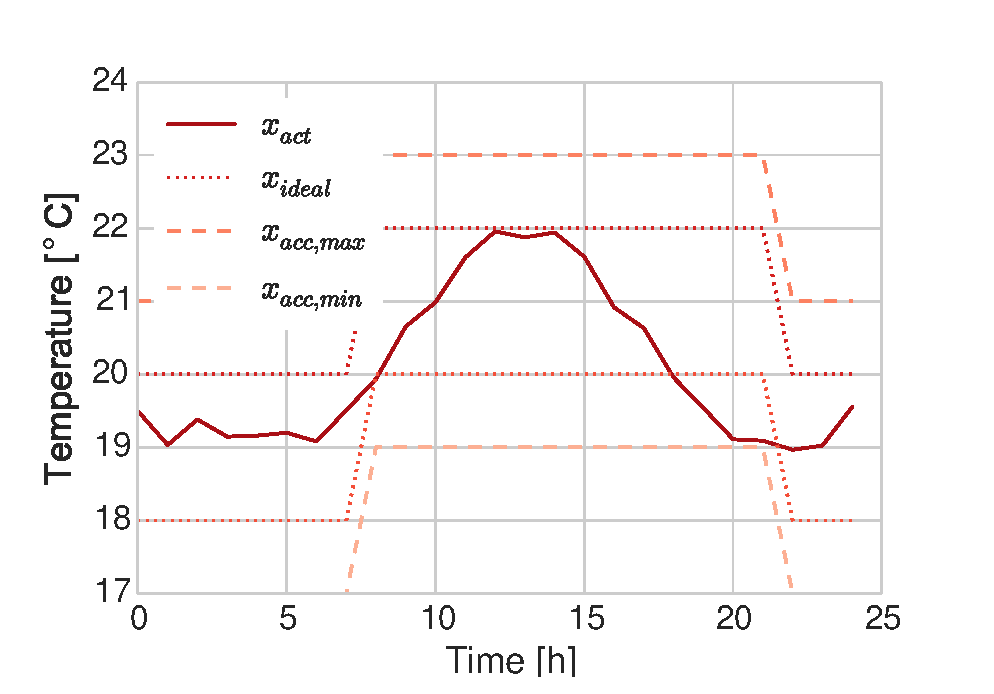
\includegraphics[width = \columnwidth]{SEGAN/tempband.eps}
\caption{Simulation of the indoor temperature of a Danish household.}
\label{fig:tempband}
\end{figure}

\begin{figure}
\centering
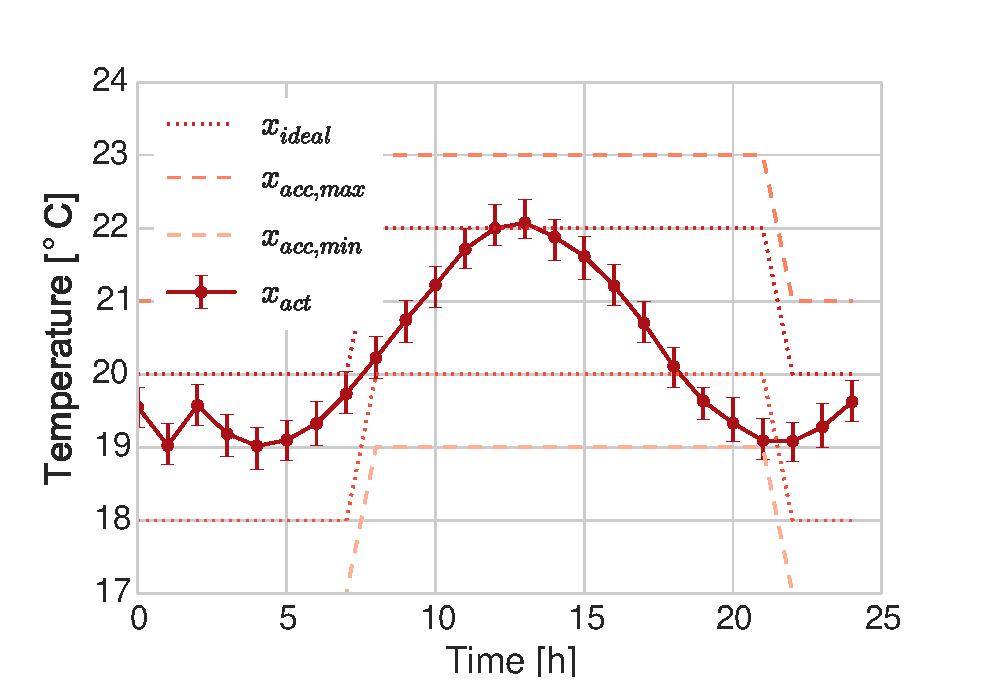
\includegraphics[width = \columnwidth]{SEGAN/tempbandclustererror.eps}
\caption{Simulation of the indoor temperature of 20 Danish households. The mean temperature is plotted, along with the minimum and maximum values of the cluster.}
\label{fig:tempbandclustererror}
\end{figure}


\section{Conclusion}\label{sec:conclusion}
\section{Conclusion and Future Work}
This work presents an initial approach to establishing a methodology for designing aggregator validation tests. This method differs from the traditional generator certification tests in that it must be carried out in simulations, so that the stochasticity of the real world disturbances affecting the aggregator can be taken into account. A drawback of this method is that it relies on the accuracy and complexity of the simulation models. This means that the components of the validation tests must be validated against reality. The test method was shown through a simplified case study on an existing aggregator. While the example shows a fictive TSO applying the test to a fictive aggregator, there is the possibility that validation of aggregators in the future will be carried out by third party test companies. 

There are still several open issues that need to be investigated with regards to aggregator validation. For example, the definition of the operation scenarios was only briefly discussed, and heuristics must be developed in order to define scenarios that are effective when testing aggregators.

An important step for the development of the validation method is the implementation of a complete test architecture with validated component models. With such a simulation framework, with realistic communication and DER models, communication delays can be implemented in order to test aggregators for time responsiveness. 

Finally, the method should be expanded to cover other ancillary services, such as voltage regulation.

We consider the work presented here an important element of enabling aggregators in the smart grid, thus enabling consumption to actively participate in the secure operation of the power system. This will help the integration of renewable energy sources into the power system.


\section*{Acknowledgment}
Parts of this work are supported by the Programme for Energy Technology Development and Demonstration (EUDP) through PowerLabDK and Innovation Fund Denmark through the iPower project. The authors thank Antonio Zecchino and Henrik W. Bindner for reviewing the draft of the paper.


\bibliographystyle{elsarticle-num}
\bibliography{bib/references.bib}
%
\end{document}


